\chapter{Free-Space Path Loss (FSPL)}
\label{ch:fspl}

\begin{nontechnical}
\textbf{Like shouting across a field}---the farther away, the quieter. Radio waves spread out and weaken with distance.

\textbf{Key insights:}
\begin{itemize}
\item \textbf{Double the distance} = signal becomes \textbf{4$\times$ weaker}
\item \textbf{Higher frequency} (5G) = weaker than lower frequency (4G) over same distance
\item \textbf{Satellites 36,000 km away}: Signal weakens by 10 trillion trillion times! (That's why dishes are big)
\end{itemize}

\textbf{Real examples:} WiFi weakens 10,000$\times$ over 50 meters. Cell towers need to be closer for 5G than 4G.
\end{nontechnical}

\section{Overview}

\textbf{Free-Space Path Loss (FSPL)} quantifies the attenuation of electromagnetic signal power as it propagates through free space (vacuum or air without obstacles). Unlike material absorption, FSPL is purely geometric---power spreads over an expanding spherical wavefront, causing the signal density to decrease with the square of distance.

\begin{keyconcept}
FSPL increases as \textbf{20 dB per decade of distance} and \textbf{20 dB per decade of frequency}. This fundamental relationship determines the feasibility of wireless communication over any given distance.
\end{keyconcept}

Understanding FSPL is critical for link budget analysis in satellite communications, cellular networks, WiFi, radar, and all wireless systems.

\section{The Friis Transmission Equation}
\label{sec:friis-equation}

The \textbf{Friis transmission equation} relates the received power to transmitted power in a free-space line-of-sight radio link:

\begin{equation}
P_R = P_T \cdot G_T \cdot G_R \cdot \left(\frac{\lambda}{4\pi d}\right)^2
\label{eq:friis}
\end{equation}

\begin{equation}
P_R = P_T \cdot G_T \cdot G_R \cdot \left(\frac{\lambda}{4\pi d}\right)^2
\end{equation}
where:
\begin{itemize}
\item $P_R$ = received power (W)
\item $P_T$ = transmitted power (W)
\item $G_T$ = transmit antenna gain (linear, dimensionless)
\item $G_R$ = receive antenna gain (linear, dimensionless)
\item $\lambda$ = wavelength (m), where $\lambda = c/f$
\item $d$ = distance between antennas (m)
\item $c$ = speed of light ($3 \times 10^8$ m/s)
\item $f$ = frequency (Hz)
\end{itemize}

\subsection{Physical Interpretation}

The Friis equation can be visualized as power spreading over a sphere:

\begin{center}
\begin{tikzpicture}[scale=1.2]
% Transmitter
\node[draw, circle, fill=black!20, minimum size=0.8cm] (tx) at (0,0) {\sffamily\small TX};
\node[below=2pt] at (tx.south) {\sffamily\scriptsize $P_T$};

% Expanding spherical wavefronts
\foreach \r/\op in {1/0.6, 2/0.4, 3/0.25, 4/0.15} {
    \draw[thick, black!\op*100] (tx) circle (\r);
}

% Power density annotations
\draw[->, thick, NavyBlue] (0,0) -- (1.5,1.5) node[midway, above left, font=\scriptsize] {$d$};
\node[draw, circle, fill=NavyBlue!20, minimum size=0.6cm] (rx) at (4,0) {\sffamily\small RX};

% Surface area annotation
\draw[<->, thick, red] (4,-0.3) arc (-90:90:0.3) node[midway, right, font=\scriptsize] {$A = 4\pi d^2$};

% Power density formula
\node[font=\scriptsize, align=center] at (2, -2) {
  Power density at distance $d$:\\
  $S = \frac{P_T G_T}{4\pi d^2}$ (W/m$^2$)
};
\end{tikzpicture}
\end{center}

\textbf{Key insight:} The transmit antenna radiates power $P_T G_T$ into a sphere of surface area $A = 4\pi d^2$. The power density at distance $d$ is:
\begin{equation}
S = \frac{P_T G_T}{4\pi d^2} \quad \text{(W/m}^2\text{)}
\label{eq:power-density}
\end{equation}

The receiving antenna captures power proportional to its effective aperture $A_{\text{eff}} = G_R \lambda^2 / (4\pi)$:
\begin{equation}
P_R = S \cdot A_{\text{eff}} = \frac{P_T G_T}{4\pi d^2} \cdot \frac{G_R \lambda^2}{4\pi} = P_T G_T G_R \left(\frac{\lambda}{4\pi d}\right)^2
\end{equation}

This derivation shows that FSPL is \textbf{not energy loss}---it is geometric spreading.

\subsection{Assumptions}

\begin{warningbox}
The Friis equation requires the following conditions:
\begin{itemize}
\item \textbf{Free space:} No obstacles, reflections, or absorbing medium
\item \textbf{Far-field region:} $d \gg \lambda$ and $d \gg$ antenna dimensions
\item \textbf{Polarization matched:} TX and RX antennas have aligned polarization
\item \textbf{Antennas aligned:} Boresight pointing directly at each other
\end{itemize}

Violations of these assumptions result in additional losses beyond FSPL.
\end{warningbox}

\section{Path Loss Definition}
\label{sec:path-loss}

\textbf{Path loss} (L) is defined as the ratio of transmitted power to received power:
\begin{equation}
L = \frac{P_T}{P_R}
\label{eq:path-loss}
\end{equation}

In decibels:
\begin{equation}
L_{\text{dB}} = 10\log_{10}(L) = 10\log_{10}\left(\frac{P_T}{P_R}\right) = P_T[\text{dBm}] - P_R[\text{dBm}]
\label{eq:path-loss-db}
\end{equation}

\subsection{FSPL Formula Derivation}

From the Friis equation~\eqref{eq:friis} with isotropic antennas ($G_T = G_R = 1$):
\begin{equation}
L = \frac{P_T}{P_R} = \left(\frac{4\pi d}{\lambda}\right)^2
\label{eq:fspl-linear}
\end{equation}

Substituting $\lambda = c/f$ and converting to decibels:
\begin{align}
\text{FSPL}_{\text{dB}} &= 20\log_{10}\left(\frac{4\pi d}{\lambda}\right) \nonumber \\
&= 20\log_{10}(4\pi) + 20\log_{10}(d) + 20\log_{10}(f) - 20\log_{10}(c) \nonumber \\
&= 20\log_{10}(d) + 20\log_{10}(f) - 147.55
\label{eq:fspl-derivation}
\end{align}

\subsection{Practical FSPL Formulas}

\textbf{SI units} (frequency in Hz, distance in meters):
\begin{equation}
\boxed{\text{FSPL}_{\text{dB}} = 20\log_{10}(d) + 20\log_{10}(f) + 92.45}
\label{eq:fspl-si}
\end{equation}

\textbf{Engineering units} (frequency in MHz, distance in km):
\begin{equation}
\boxed{\text{FSPL}_{\text{dB}} = 20\log_{10}(d_{\text{km}}) + 20\log_{10}(f_{\text{MHz}}) + 32.45}
\label{eq:fspl-eng}
\end{equation}

\begin{calloutbox}{Choosing the Right Formula}
Use equation~\eqref{eq:fspl-si} for theoretical calculations (maintains dimensional consistency). Use equation~\eqref{eq:fspl-eng} for practical link budgets (matches typical engineering units).

The constant term differs because:
\begin{itemize}
\item $92.45 = 20\log_{10}(4\pi/c)$ where $c = 3\times10^8$ m/s
\item $32.45 = 92.45 - 20\log_{10}(10^6) - 20\log_{10}(10^3)$
\end{itemize}
\end{calloutbox}

\section{Worked Examples}
\label{sec:examples}

\subsection{Example 1: WiFi Link (2.4 GHz, 10 m)}

\textbf{Given:}
\begin{itemize}
\item Frequency: $f = 2.4$ GHz $= 2.4 \times 10^9$ Hz
\item Distance: $d = 10$ m
\end{itemize}

\textbf{Solution:} Using equation~\eqref{eq:fspl-si}:
\begin{align}
\text{FSPL}_{\text{dB}} &= 20\log_{10}(10) + 20\log_{10}(2.4 \times 10^9) + 92.45 \nonumber \\
&= 20 + 187.6 + 92.45 \nonumber \\
&= 100.05 \text{ dB}
\end{align}

\textbf{Interpretation:} Signal power drops by a factor of $10^{10}$ (10 billion) over 10 m! This demonstrates why WiFi requires relatively high transmit power despite short distances.

\subsection{Example 2: Cellular Link (900 MHz, 1 km)}

\textbf{Given:}
\begin{itemize}
\item Frequency: $f = 900$ MHz $= 0.9$ GHz
\item Distance: $d = 1$ km
\end{itemize}

\textbf{Solution:} Using equation~\eqref{eq:fspl-eng}:
\begin{align}
\text{FSPL}_{\text{dB}} &= 20\log_{10}(1) + 20\log_{10}(900) + 32.45 \nonumber \\
&= 0 + 59.1 + 32.45 \nonumber \\
&= 91.55 \text{ dB}
\end{align}

\textbf{Note:} At 1000 m using SI formula: $20\log_{10}(1000) + 20\log_{10}(9\times10^8) + 92.45 = 60 + 179.1 + 92.45 = 131.55$ dB. Wait, let me recalculate: $20\log_{10}(9\times10^8) = 20(8.954) = 179.08$, giving total 131.53 dB.

\subsection{Example 3: GEO Satellite (12 GHz, 36,000 km)}

\textbf{Given:}
\begin{itemize}
\item Frequency: $f = 12$ GHz (Ku-band downlink)
\item Distance: $d = 36{,}000$ km (geostationary orbit)
\end{itemize}

\textbf{Solution:} Using equation~\eqref{eq:fspl-eng}:
\begin{align}
\text{FSPL}_{\text{dB}} &= 20\log_{10}(36{,}000) + 20\log_{10}(12{,}000) + 32.45 \nonumber \\
&= 91.1 + 81.6 + 32.45 \nonumber \\
&= 205.2 \text{ dB}
\end{align}

\begin{calloutbox}{Satellite Link Challenge}
\textbf{Massive loss!} 205 dB means received power is $10^{-20.5}$ times transmitted power. This extreme attenuation requires:
\begin{itemize}
\item High transmit power (10--200 W)
\item High-gain antennas (30--50 dBi on satellite, 35--45 dBi on ground)
\item Low-noise amplifiers (LNAs) at receiver
\item Forward error correction (FEC) coding
\end{itemize}
\end{calloutbox}

\subsection{Example 4: THz Link (1 THz, 10 m)}

\textbf{Given:}
\begin{itemize}
\item Frequency: $f = 1$ THz $= 10^{12}$ Hz
\item Distance: $d = 10$ m
\end{itemize}

\textbf{Solution:} Using equation~\eqref{eq:fspl-si}:
\begin{align}
\text{FSPL}_{\text{dB}} &= 20\log_{10}(10) + 20\log_{10}(10^{12}) + 92.45 \nonumber \\
&= 20 + 240 + 92.45 \nonumber \\
&= 352.45 \text{ dB}
\end{align}

\textbf{Extreme loss!} This demonstrates why terahertz communications are inherently short-range. Even without atmospheric absorption, FSPL alone exceeds 350 dB at modest distances.

\section{Scaling Laws}
\label{sec:scaling-laws}

\subsection{Distance Dependence}

FSPL follows an inverse-square law in linear units:
\begin{equation}
\text{FSPL} \propto d^2 \quad \text{(power law)}
\end{equation}

In decibels, this becomes a logarithmic relationship:
\begin{equation}
\text{FSPL}_{\text{dB}} \text{ increases by 20 dB per decade of distance}
\end{equation}

\textbf{Examples:}
\begin{itemize}
\item $1 \text{ m} \rightarrow 10 \text{ m}$: +20 dB loss
\item $10 \text{ m} \rightarrow 100 \text{ m}$: +20 dB loss
\item $100 \text{ m} \rightarrow 1 \text{ km}$: +20 dB loss
\end{itemize}

\textbf{Doubling distance:} +6 dB loss (power drops to 1/4)

\subsection{Frequency Dependence}

FSPL also follows an inverse-square law with frequency:
\begin{equation}
\text{FSPL} \propto f^2 \quad \text{(power law)}
\end{equation}

In decibels:
\begin{equation}
\text{FSPL}_{\text{dB}} \text{ increases by 20 dB per decade of frequency}
\end{equation}

\textbf{Examples:}
\begin{itemize}
\item $100 \text{ MHz} \rightarrow 1 \text{ GHz}$: +20 dB loss
\item $1 \text{ GHz} \rightarrow 10 \text{ GHz}$: +20 dB loss
\item $10 \text{ GHz} \rightarrow 100 \text{ GHz}$: +20 dB loss
\end{itemize}

\textbf{Doubling frequency:} +6 dB loss (higher frequencies experience more path loss)

\textbf{Why?} The effective aperture of a receiving antenna is proportional to $\lambda^2 = (c/f)^2$. Higher frequencies have shorter wavelengths, resulting in smaller effective aperture and thus lower received power.

\subsection{Path Loss vs Distance}

The following diagram shows FSPL as a function of distance for various frequencies:

\begin{center}
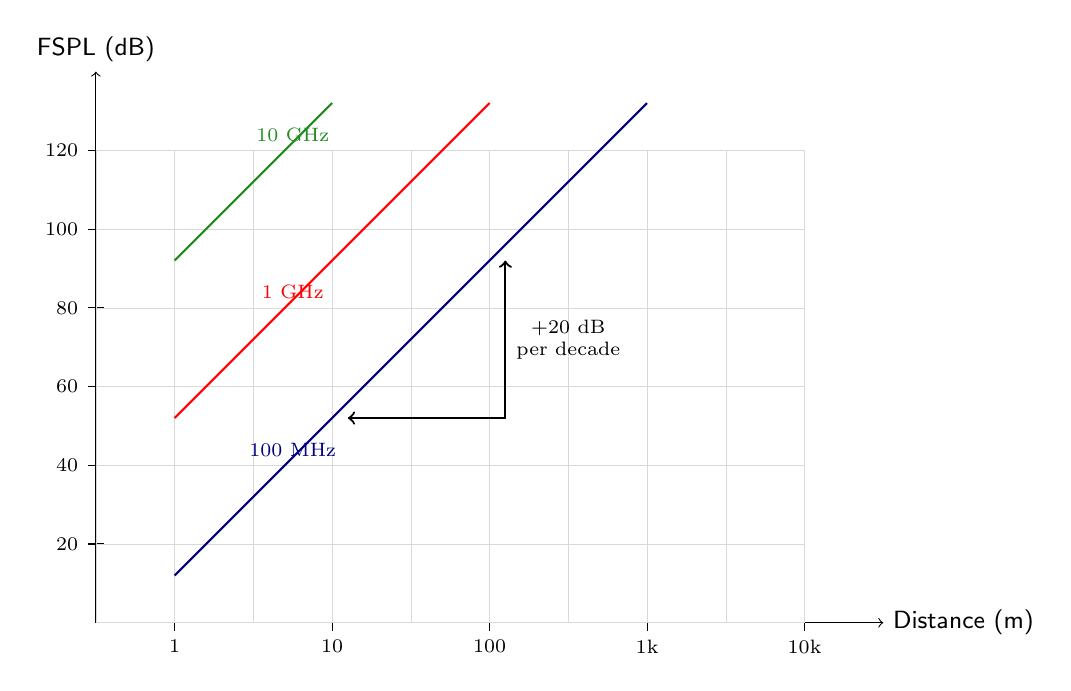
\begin{tikzpicture}[scale=1.0]
% Axes
\draw[->] (0,0) -- (10,0) node[right] {\sffamily\small Distance (m)};
\draw[->] (0,0) -- (0,7) node[above] {\sffamily\small FSPL (dB)};

% X-axis labels (logarithmic scale)
\foreach \x/\label in {1/1, 3/10, 5/100, 7/1k, 9/10k} {
    \draw (\x,0.1) -- (\x,-0.1) node[below, font=\scriptsize] {\label};
}

% Y-axis labels
\foreach \y/\label in {1/20, 2/40, 3/60, 4/80, 5/100, 6/120} {
    \draw (0.1,\y) -- (-0.1,\y) node[left, font=\scriptsize] {\label};
}

% Grid
\draw[very thin, gray!30] (0,0) grid (9,6);

% Plot lines for different frequencies
% 100 MHz (blue)
\draw[thick, NavyBlue] (1,0.6) -- (3,2.6) -- (5,4.6) -- (7,6.6);
\node[NavyBlue, font=\scriptsize] at (2.5, 2.2) {100 MHz};

% 1 GHz (red)
\draw[thick, red] (1,2.6) -- (3,4.6) -- (5,6.6);
\node[red, font=\scriptsize] at (2.5, 4.2) {1 GHz};

% 10 GHz (green)
\draw[thick, ForestGreen] (1,4.6) -- (3,6.6);
\node[ForestGreen, font=\scriptsize] at (2.5, 6.2) {10 GHz};

% Slope annotation (20 dB/decade)
\draw[<->, thick, black] (3.2, 2.6) -- (5.2, 2.6) -- (5.2, 4.6);
\node[font=\scriptsize, align=center] at (6, 3.6) {+20 dB\\per decade};
\end{tikzpicture}
\end{center}

\textbf{Observations:}
\begin{enumerate}
\item All curves have identical slope (20 dB/decade)
\item Higher frequencies have uniformly higher path loss
\item Doubling distance or frequency adds 6 dB loss
\end{enumerate}

\section{Physical Interpretation: Not True ``Loss''}
\label{sec:physical-interpretation}

\begin{keyconcept}
FSPL is \textbf{NOT} energy dissipation---free space is lossless! It represents \textbf{geometric spreading}: the same total radiated power distributes over an ever-expanding spherical wavefront.
\end{keyconcept}

Consider a transmit antenna radiating power $P_T G_T$ isotropically. At distance $d$, this power is spread over a sphere of surface area:
\begin{equation}
A_{\text{sphere}} = 4\pi d^2
\end{equation}

The power density (power flux) at distance $d$ is:
\begin{equation}
S = \frac{P_T G_T}{4\pi d^2} \quad \text{(W/m}^2\text{)}
\end{equation}

The receiving antenna captures power proportional to its effective aperture:
\begin{equation}
A_{\text{eff}} = \frac{G_R \lambda^2}{4\pi}
\end{equation}

Therefore, received power is:
\begin{equation}
P_R = S \cdot A_{\text{eff}} = \frac{P_T G_T}{4\pi d^2} \cdot \frac{G_R \lambda^2}{4\pi} = P_T G_T G_R \left(\frac{\lambda}{4\pi d}\right)^2
\end{equation}

This recovers the Friis equation~\eqref{eq:friis}.

\textbf{Analogy:} Like a flashlight beam spreading out---the same total power illuminates a larger area at greater distance, reducing intensity but not destroying energy.

\section{Link Budget Analysis}
\label{sec:link-budget}

A \textbf{link budget} accounts for all gains and losses in a communication link:

\begin{equation}
\boxed{P_R[\text{dBm}] = P_T[\text{dBm}] + G_T[\text{dBi}] + G_R[\text{dBi}] - \text{FSPL}[\text{dB}] - L_{\text{other}}[\text{dB}]}
\label{eq:link-budget}
\end{equation}

where:
\begin{itemize}
\item $P_T$ = transmit power (dBm, referenced to 1 mW)
\item $G_T, G_R$ = antenna gains (dBi, referenced to isotropic)
\item FSPL = free-space path loss (dB)
\item $L_{\text{other}}$ = additional losses (cables, connectors, atmosphere, etc.)
\end{itemize}

\textbf{Design goal:} Ensure $P_R \gg P_{\text{noise}}$ (receiver noise floor) for reliable communication.

\subsection{Link Budget Diagram}

\begin{center}
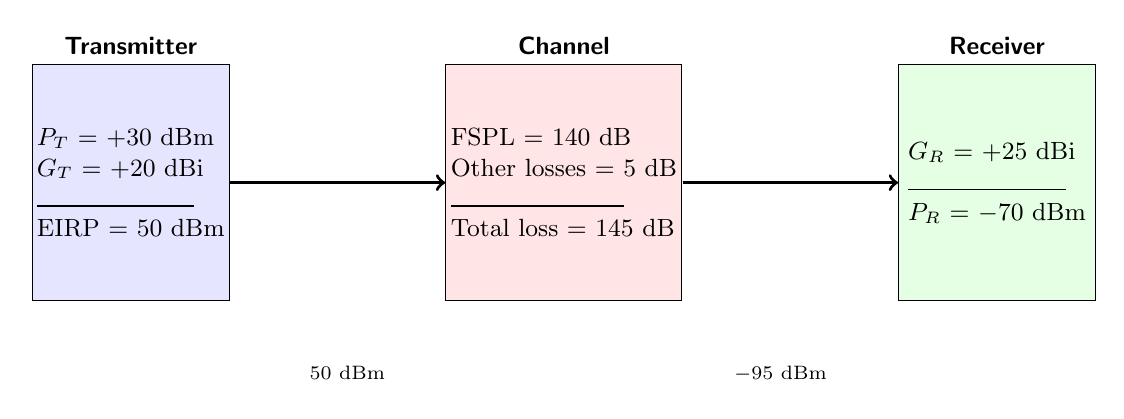
\begin{tikzpicture}[scale=1.1, font=\small]
% Transmitter box
\node[draw, rectangle, minimum width=2.5cm, minimum height=3cm, fill=blue!10] (tx) at (0,0) {};
\node[above] at (tx.north) {\sffamily\bfseries Transmitter};
\node[align=left] at (tx.center) {
  $P_T$ = +30 dBm\\
  $G_T$ = +20 dBi\\
  \rule{2cm}{0.4pt}\\
  EIRP = 50 dBm
};

% Channel box
\node[draw, rectangle, minimum width=3cm, minimum height=3cm, fill=red!10] (ch) at (5,0) {};
\node[above] at (ch.north) {\sffamily\bfseries Channel};
\node[align=left] at (ch.center) {
  FSPL = 140 dB\\
  Other losses = 5 dB\\
  \rule{2.2cm}{0.4pt}\\
  Total loss = 145 dB
};

% Receiver box
\node[draw, rectangle, minimum width=2.5cm, minimum height=3cm, fill=green!10] (rx) at (10,0) {};
\node[above] at (rx.north) {\sffamily\bfseries Receiver};
\node[align=left] at (rx.center) {
  $G_R$ = +25 dBi\\
  \rule{2cm}{0.4pt}\\
  $P_R$ = $-70$ dBm
};

% Arrows
\draw[->, very thick] (tx.east) -- (ch.west);
\draw[->, very thick] (ch.east) -- (rx.west);

% Power flow annotation
\node[below, font=\scriptsize] at (2.5, -2) {50 dBm};
\node[below, font=\scriptsize] at (7.5, -2) {$-95$ dBm};
\end{tikzpicture}
\end{center}

\subsection{Worked Example: WiFi Link Budget (2.4 GHz, 50 m)}

\textbf{Scenario:} Indoor WiFi access point to laptop

\textbf{Transmitter:}
\begin{itemize}
\item TX power: $P_T = +20$ dBm (100 mW, typical WiFi)
\item TX antenna gain: $G_T = +2$ dBi (dipole)
\item EIRP: $20 + 2 = 22$ dBm
\end{itemize}

\textbf{Channel:}
\begin{itemize}
\item Distance: $d = 50$ m
\item Frequency: $f = 2.4$ GHz $= 2400$ MHz
\item FSPL (using engineering units):
\begin{equation}
\text{FSPL} = 20\log_{10}(0.05) + 20\log_{10}(2400) + 32.45 = -26.0 + 67.6 + 32.45 = 74.1 \text{ dB}
\end{equation}
\item Indoor losses (walls, furniture): $\sim$15 dB
\item Total channel loss: $74.1 + 15 = 89.1$ dB
\end{itemize}

\textbf{Receiver:}
\begin{itemize}
\item RX antenna gain: $G_R = +2$ dBi
\item Cable loss: $-1$ dB
\item Net RX gain: $+1$ dB
\end{itemize}

\textbf{Received power:}
\begin{equation}
P_R = 22 + 1 - 89.1 = -66.1 \text{ dBm}
\end{equation}

\textbf{Noise floor:} For bandwidth $B = 20$ MHz at room temperature ($T = 300$ K):
\begin{equation}
N = -174 + 10\log_{10}(2 \times 10^7) = -174 + 73 = -101 \text{ dBm}
\end{equation}

\textbf{SNR:}
\begin{equation}
\text{SNR} = P_R - N = -66.1 - (-101) = 34.9 \text{ dB}
\end{equation}

\begin{calloutbox}{Link Assessment}
\textbf{Result:} Link closes successfully with 35 dB SNR, which is excellent for WiFi. This provides sufficient margin for:
\begin{itemize}
\item High-order modulation (64-QAM or higher)
\item High data rates (up to 100+ Mbps)
\item Fading margin and interference tolerance
\end{itemize}

Typical WiFi receivers require $\sim -65$ dBm minimum sensitivity, so this link has 1 dB margin.
\end{calloutbox}

\section{Real-World Deviations from FSPL}
\label{sec:deviations}

\subsection{FSPL Assumes Ideal Free Space}

\begin{warningbox}
FSPL is valid only in ideal conditions:
\begin{itemize}
\item \textbf{No obstacles:} Direct line-of-sight
\item \textbf{No atmosphere:} Vacuum or perfectly transparent medium
\item \textbf{No multipath:} Single direct ray, no reflections
\item \textbf{No weather:} No rain, fog, or atmospheric turbulence
\end{itemize}

In reality, \textbf{actual path loss $>$ FSPL} due to additional attenuation mechanisms.
\end{warningbox}

\textbf{Reality:}
\begin{itemize}
\item \textbf{Atmosphere absorbs:} Especially water vapor at mmWave/THz frequencies
\item \textbf{Obstacles block:} Buildings, trees, terrain cause diffraction and shadowing
\item \textbf{Ground reflections:} Create multipath interference
\item \textbf{Weather attenuates:} Rain fade, fog absorption
\end{itemize}

\subsection{Frequency-Specific Effects}

\textbf{Low Frequencies ($<$ 30 MHz):}
\begin{itemize}
\item Ground wave propagation along Earth's surface
\item Ionospheric reflection (HF skip)
\item \textbf{Can exceed FSPL predictions} (longer range via non-line-of-sight paths)
\end{itemize}

\textbf{Mid Frequencies (30 MHz -- 3 GHz):}
\begin{itemize}
\item Mostly line-of-sight (LOS) propagation
\item FSPL + diffraction around obstacles
\item Close to FSPL predictions in clear conditions
\end{itemize}

\textbf{High Frequencies ($>$ 3 GHz):}
\begin{itemize}
\item Atmospheric absorption becomes significant
\item Rain fade (especially $>$ 10 GHz)
\item \textbf{Path loss $>$ FSPL} by 5--20 dB
\end{itemize}

\textbf{THz ($>$ 300 GHz):}
\begin{itemize}
\item Extreme atmospheric absorption
\item Water vapor molecular resonances
\item \textbf{Path loss $\gg$ FSPL} (can be +100 dB additional loss!)
\end{itemize}

\subsection{Path Loss Exponent}

In non-ideal environments, measured path loss often follows:
\begin{equation}
P_R \propto d^{-n}
\label{eq:path-loss-exponent}
\end{equation}

where $n$ is the \textbf{path loss exponent}:
\begin{center}
\begin{tabular}{@{}lc@{}}
\toprule
\textbf{Environment} & \textbf{Path Loss Exponent ($n$)} \\
\midrule
Free space & 2.0 \\
Urban macrocell & 3.0--4.0 \\
Indoor office & 2.5--3.5 \\
Dense urban & 4.0--6.0 \\
Obstructed indoor & 4.0--6.0 \\
\bottomrule
\end{tabular}
\end{center}

\textbf{Empirical models} (e.g., Okumura-Hata, COST 231, 3GPP models) extend FSPL with environment-specific corrections to fit measured data.

\section{Applications}
\label{sec:applications}

\subsection{Satellite Communications}

FSPL is the dominant loss mechanism in satellite links due to extreme distances:
\begin{itemize}
\item \textbf{LEO satellites (500--2000 km):} FSPL $\sim$ 160--175 dB
\item \textbf{GEO satellites (36,000 km):} FSPL $\sim$ 195--210 dB
\item \textbf{Deep space (Mars):} FSPL $>$ 270 dB
\end{itemize}

Link design requires high-gain antennas, high transmit power, and sophisticated error correction.

\subsection{Cellular Networks}

Cell tower placement is optimized based on FSPL predictions:
\begin{itemize}
\item \textbf{Macrocells (4G/5G):} Cover 1--20 km radius, accounting for FSPL + shadowing
\item \textbf{Small cells (5G):} Higher frequency (3.5--28 GHz) = higher FSPL = closer spacing
\item \textbf{mmWave 5G:} Extreme FSPL necessitates very dense deployment (100--200 m spacing)
\end{itemize}

\subsection{WiFi and Indoor Wireless}

FSPL predicts signal strength throughout buildings:
\begin{itemize}
\item \textbf{2.4 GHz WiFi:} Lower FSPL, better range, more wall penetration
\item \textbf{5 GHz WiFi:} Higher FSPL (+6 dB vs 2.4 GHz), shorter range, more capacity
\item \textbf{6 GHz WiFi (WiFi 6E):} Even higher FSPL, densest deployment
\end{itemize}

\subsection{Radar and Sensing}

Radar systems experience \textbf{two-way FSPL} (signal travels to target and back):
\begin{equation}
\text{FSPL}_{\text{radar}} = 2 \times \text{FSPL}_{\text{one-way}} = 40\log_{10}(d) + 40\log_{10}(f) + \text{const}
\end{equation}

This $d^4$ dependence severely limits radar range at high frequencies.

\subsection{Free-Space Optical (FSO) Communications}

FSO links (infrared/visible light) follow FSPL at optical frequencies:
\begin{itemize}
\item $f \sim 10^{14}$ Hz $\rightarrow$ wavelength $\sim$ 1--10 $\mu$m
\item FSPL at 1 km: $\sim$ 280 dB (even higher than THz!)
\item Requires laser beams with extremely narrow divergence angles
\end{itemize}

\section{Summary}
\label{sec:summary}

\begin{center}
\begin{tabular}{@{}ll@{}}
\toprule
\textbf{Parameter} & \textbf{Value/Description} \\
\midrule
Physical mechanism & Geometric spreading of spherical wavefront \\
Distance dependence & $\propto d^2$ (20 dB/decade) \\
Frequency dependence & $\propto f^2$ (20 dB/decade) \\
FSPL formula (SI) & $20\log_{10}(d) + 20\log_{10}(f) + 92.45$ dB \\
FSPL formula (eng) & $20\log_{10}(d_{\text{km}}) + 20\log_{10}(f_{\text{MHz}}) + 32.45$ dB \\
Doubling distance & +6 dB loss \\
Doubling frequency & +6 dB loss \\
Energy dissipation & None (lossless) \\
Typical application & Link budget baseline for all wireless systems \\
\bottomrule
\end{tabular}
\end{center}

\begin{keyconcept}
\textbf{Key Takeaways:}
\begin{enumerate}
\item \textbf{FSPL $\propto d^2 \cdot f^2$:} Geometric spreading, worse at high frequencies
\item \textbf{20 dB per decade:} Doubling $d$ or $f$ adds 6 dB loss
\item \textbf{Not energy loss:} Power spreads out, doesn't vanish
\item \textbf{Baseline for link budgets:} Real losses are usually higher
\item \textbf{Frequency trade-off:} Higher $f$ $\rightarrow$ more bandwidth but more path loss
\item \textbf{THz communications:} FSPL alone is $\sim$350 dB at 10 m, 1 THz!
\end{enumerate}
\end{keyconcept}

\section{Further Reading}
\label{sec:further-reading}

\begin{itemize}
\item \textbf{Chapter~\ref{ch:antenna-basics}:} Antenna Theory Basics---antenna gain ($G_T$, $G_R$)
\item \textbf{Chapter~\ref{ch:snr}:} Signal-to-Noise Ratio---FSPL vs additive noise
\item \textbf{Chapter~\ref{ch:atmospheric-effects}:} Atmospheric Effects---additional losses beyond FSPL
\item \textbf{Chapter~\ref{ch:channel-models}:} Channel Models (Rayleigh \& Rician)---deviations from FSPL
\item \textbf{Chapter~\ref{ch:thz}:} Terahertz Technology---extreme FSPL regime
\item \textbf{Chapter~\ref{ch:maxwell}:} Maxwell's Equations \& Wave Propagation---theoretical foundation
\end{itemize}

\section{References}
\label{sec:references}

\begin{enumerate}
\item \textbf{Friis, H.T.} (1946) ``A note on a simple transmission formula'' \textit{Proc. IRE} 34, 254--256
\item \textbf{Rappaport, T.S.} (2002) \textit{Wireless Communications: Principles and Practice} 2nd ed. (Prentice Hall)
\item \textbf{Goldsmith, A.} (2005) \textit{Wireless Communications} (Cambridge University Press)
\item \textbf{ITU-R P.525} (2019) ``Calculation of free-space attenuation''
\item \textbf{Proakis, J.G. \& Salehi, M.} (2008) \textit{Digital Communications} 5th ed. (McGraw-Hill)
\end{enumerate}
